\documentclass{beamer}
\usepackage{tikz}
\usepackage{filecontents}
\begin{filecontents}{\jobname-picture.tex}
  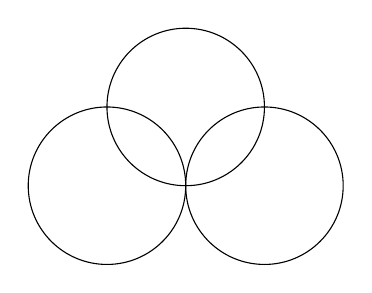
\begin{tikzpicture}
    \draw (0,0) circle (1);
    \uncover<2->{
      \draw (2,0) circle (1);}
    \uncover<3->{
      \draw (1,1) circle (1);}
  \end{tikzpicture}
\end{filecontents}

\begin{document}

  \begin{frame}{The Picture}
    Some text
    \begin{center}
      \input{\jobname-picture}
    \end{center}
  \end{frame}

  \begin{frame}<2>{Conclusion}
    \centering
    \input{\jobname-picture}
  \end{frame}

\end{document}
